\chapter{Developed Tools}

This chapter contains an overview of why supplementary tools were deemed necessary for an already working reduction process (\S~\ref{sec:polsalt_limits}), which aspects of the reduction process have been altered, replaced, or added (\S~\ref{sec:mod_tools}, \ref{sec:add_tools}), and finally what an updated reduction process consists of using a combination of all software (\S~\ref{sec:red_proc}).


\section{Limitations of POLSALT and the Need for a Supplementary Tool} \label{sec:polsalt_limits} % Rename

% Why
The creation of supplementary tools for \polsalt\ spectropolarimetric reductions stem from, primarily, the limitations of the wavelength calibration process and a need for a way to compare wavelength solutions across matching $O$ and $E$ polarization beams. Due to the time-consuming process of recalibrating the wavelength solutions it is not feasible to perform the wavelength calibrations time and time again for any amount of reductions larger than a handful of observations.
\prgph

% PG0300 reasoning
The prime motivation of finding an alternate method of wavelength calibrating the data stemmed from a large backlog of unused data taken using the $PG0300$. The only arc available for the $PG0300$ with a close enough articulation and grating angle ($\sim 10.68$ and $\sim 5.38$, respectively) was \gls{SALT}'s Argon lamp which displayed sparse spectral features with large gaps over the wavelength range at these grating and articulation angles. This often lead to inconsistent wavelength solutions, or failed altogether, through \polsalt, since minor deviations of identified spectral features may result in large deviations in regions with no spectral features.
\prgph

% How
The chosen solution was to use a well established tool to perform the wavelength calibration - one which allows for rapid recalibrations as well as provides a familiar interface with which the user can analyze their wavelength solutions. \iraf\ provides this familiar environment and reliability, even considering it's age and \hyperlink{https://github.com/iraf-community/iraf}{limited community development}. Unfortunately, \iraf\ is unable to natively parse the file structure implemented by \polsalt\ `as is' and formatting of the data structures are necessary for integration purposes. This restructuring works both ways as once the \iraf\ reductions are complete the format must be reformatted to match that of the \polsalt\ output such that the reduction process may carry on in \polsalt.
\prgph

\begin{figure}[t]
    \centering
    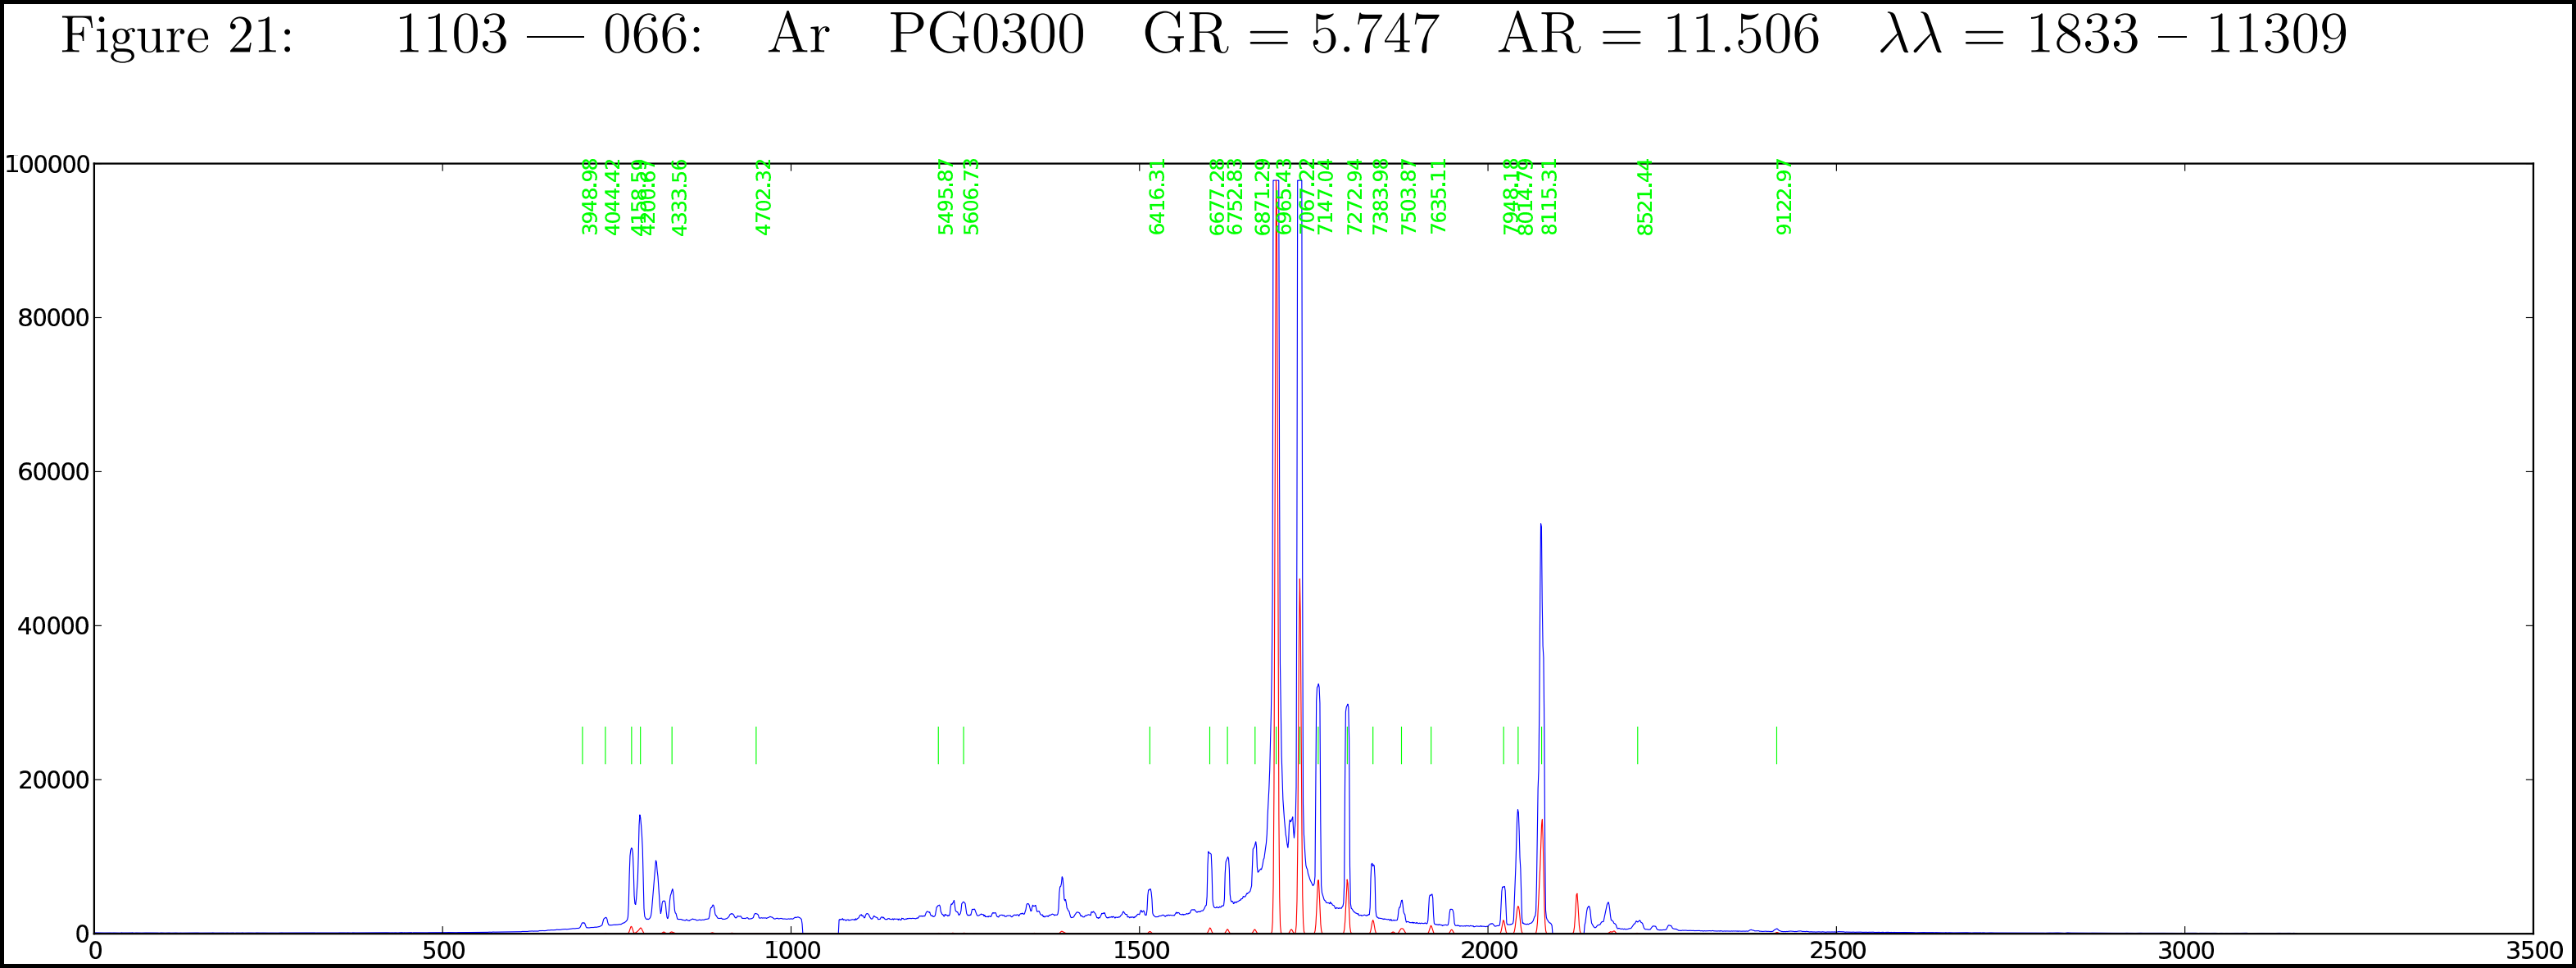
\includegraphics[width = 0.98\textwidth]{figures/3_arc_spectrum.png}
    \caption{One of many Argon arc lamp spectra as provided by \gls{SALT} for line identification. Plot adapted from \gls{SALT}'s published Longslit Line Atlases (as of 2024),\protect\footnotemark resized to fit within the document margins but otherwise unchanged.}
    \label{fig:ar_arc_salt}
\end{figure}
\footnotetext{\protect\href{https://pysalt.salt.ac.za/lineatlas/plot_line_argon_lores.pdf}{`low resolution' Ar plot} sourced from \protect\url{https://astronomers.salt.ac.za/data/salt-longslit-line-atlas/}}


\section{Wavelength calibrations - Supplementary Tools and IRAF} \label{sec:mod_tools}

The supplementary tools offer an alternate procedure for wavelength calibrations for the \polsalt\ pipeline. This procedure can be broken into three unique steps: the parsing of \polsalt\ data into an \iraf\ friendly format, referred to as splitting; the wavelength calibration performed in \iraf; and the reformatting of the data with its wavelength calibration back into the format expected by \polsalt, referred to as joining.

\begin{figure}[t]
    \centering
    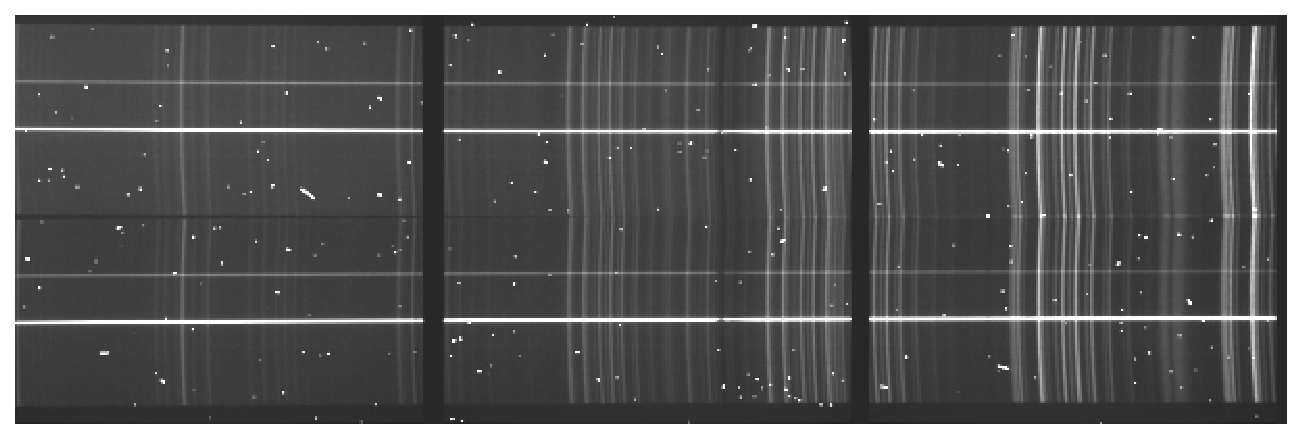
\includegraphics[width = 1.0\textwidth]{figures/3_pre_wav_cal.pdf}
    \caption{The science extension of a typical \polsalt\ \acs{FITS} file after basic \gls{CCD} reductions have been completed.}
    \label{fig:polsalt_pre_wav_cal}
\end{figure}


\subsection{Splitting the POLSALT pre-calibration files}

% Why necessary
%   Mention steps before and how they return (especially) the file structure.
As mentioned previously, the format of the \gls{FITS} file created by \polsalt\ after basic \gls{CCD} reductions and that expected by \iraf\ to be used for the wavelength calibrations are incompatible. A typical \gls{FITS} file created by the \polsalt\ basic \gls{CCD} reductions process contains a primary header along with the various image extensions, all of which include the trace for both polarimetry beams, as seen in Figure~\ref{fig:polsalt_pre_wav_cal}. \iraf\ deals best with a singular trace, and therefore a singular polarization beam, at a time.
\prgph

In an attempt to simplify the \iraf\ reduction procedure it was decided to split the polarization beams into their own files, as the parameters of \iraf\ tasks generally handle lists of files better than subregions of the same \gls{HDU}, and generally allowed for easier calibrations further down the \iraf\ wavelength calibration process.
\prgph

% What it does -> Primary focus
%   All processes run & description of each. Focus on why.
The \polsalt\ files with basic \gls{CCD} reductions applied, namely \gls{FITS} files with the prefix `mxgbp' (\S~\ref{subsec:polsalt}), are used as the starting point for the supplementary tool's \texttt{split} method. Running \texttt{split} finds all the \gls{FITS} files for wavelength calibration within the working directory, creates two empty \gls{HDU} structures for each sub-extension of the \gls{FITS} file, and appends all science and header data necessary for wavelength calibration to the relevant \gls{HDU} structure.
\prgph

% Focus on minimizing changes and optimizing size
As the intent was always to parse the wavelength function back into \polsalt\ it was decided to keep these temporary \gls{FITS} files as light as possible. This is especially necessary when considering the amount of frames that must be taken for a single spectropolarimetric observation, and then how the number of observations increases for long term studies.
\prgph

\begin{figure}[t]
    \centering
    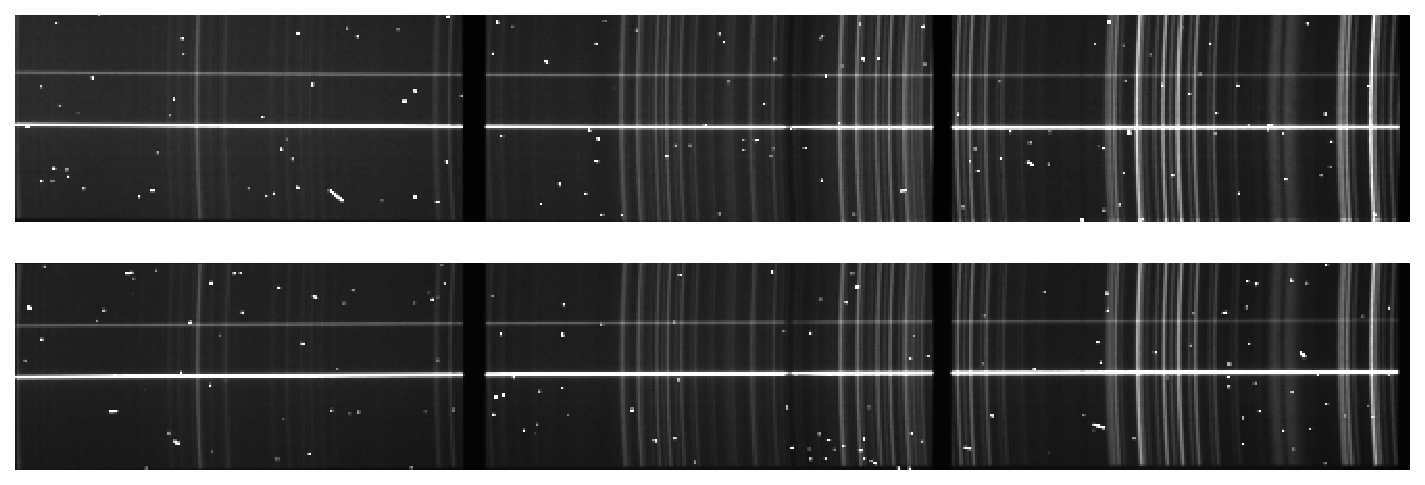
\includegraphics[width = 1.0\textwidth]{figures/3_OEsplit.pdf}
    \caption{The split $O$ and $E$ beams as handed to \iraf.}
    \label{fig:OE_split}
\end{figure}

% Any changes from how polsalt would do it
To aid the \iraf\ wavelength calibrations, row cropping and file list creation were introduced into the \texttt{split} method to ignore the regions without a trace either side of the frame, and to list the $O$ and $E$ beam \gls{FITS} files, respectively. The row cropping was decided on as \iraf\ does not handle the empty rows well, specifically when it comes to the \texttt{reidentify} task. Otherwise, defaults, such as which row to split the beams along, were kept as close to the \polsalt\ pipeline as possible.


\subsection{IRAF wavelength calibration}\label{subsec:IRAF_wav_cal}

% What is IRAF and why necessary
\iraf\ is a collection of software designed specifically for the reduction and analysis of astronomical images and spectra. The software consists of many tasks which perform specific operations and which are grouped into relevant packages. Only a brief overview of the tasks will be provided here as every researcher, university, and research group have their own preferred wavelength calibration procedures and often use specific parameters for the various \iraf\ tasks (e.g. the order and type of the polynomial used in \texttt{identify}, etc.).
\prgph

A useful \iraf\ task that will not be discussed but nevertheless deserves a mention is the \texttt{mkscript} task in the \texttt{system} package which allows a user to create and save a task along with the defined parameters as a file which can later be called as a script. It is instrumental as a scripting aid and is what allows \iraf\ its rapid recalibrations of the wavelength solutions.
\prgph

For the alternate wavelength calibrations, the relevant tasks, in order, are \texttt{identify} and \texttt{reidentify} located in the \texttt{noao.onedspec} package, and the \texttt{fitcoords} and optionally the \texttt{transform} tasks located under the \texttt{noao.twodspec.longslit} package. These tasks produce a two-dimensional wavelength solution and thus must all be run twice to create the different wavelength solutions for each of the two spectropolarimetric beams.

% What it does -> Primary focus
%   All processes run & description of each. Focus on why.
% https://astro.uni-bonn.de/~sysstw/lfa_html/iraf/noao.onedspec.identify.html#h_29
% https://iraf.net/irafdocs/formats/identify.php
\paragraph{Identify}
The \texttt{identify} task is used to interactively determine a one-dimensional wavelength function across a chosen row of an arc exposure by identifying features in the spectrum with known wavelengths. \texttt{identify} gives the first approximation of the wavelength solution, which is saved to a local database, and is built on in subsequent tasks. It is thus imperative that the initial fit is done well to minimize errors further down the calibration process.
\prgph

The process of using \texttt{identify} consists of identifying known features spanning the entire wavelength range and then removing identified features which negatively impact the wavelength solution. A balance must be found between the number of identified features and parameters of the fit against the deviation of the fit from the known features. % RMS

% https://astro.uni-bonn.de/~sysstw/lfa_html/iraf/noao.onedspec.reidentify.html#h_29
\paragraph{Reidentify}
The \texttt{reidentify} task is used to run the \texttt{identify} task autonomously and repeatedly across the entirety of the arc exposure at a defined interval. \texttt{reidentify} uses the one-dimensional wavelength solution stored in the database created by the initial \texttt{identify} call and shifts the identified points to match their known spectral features. The task may fail based on a number of defined conditions, most common of which is the loss of features as the task moves further from the row at which the user ran \texttt{identify}.
\prgph

When running \texttt{reidentify} non-interactively, it is recommended to set the \texttt{verbose} parameter to `\texttt{yes}' as this will allow immediate confirmation whether the task quit early or not. Regardless of where the task ended, the newly defined wavelength solutions are appended to the local database.

% https://astro.uni-bonn.de/~sysstw/lfa_html/iraf/noao.twodspec.longslit.fitcoords.html
% https://iraf.net/irafdocs/formats/fitcoords.php
\paragraph{Fitcoords}
The \texttt{fitcoords} task is used to combine the collection of one-dimensional wavelength solutions in the local database to a two-dimensional surface function. This surface function is the final two-dimensional wavelength solution and is what is needed to convert the \iraf\ formatted wavelength calibrated \gls{FITS} files back into the \polsalt\ format.
\prgph

The process of using \texttt{fitcoords}, follows closely to that of \texttt{identify} and consists of examining the distribution of identified points and eliminating any points that \texttt{reidentify} may have misidentified. By eliminating outliers with bad residuals and modifying the two-dimensional surface function type and degree, the overall error of the fit decreases, matching more closely to what the `true' wavelength solution is.

% https://astro.uni-bonn.de/~sysstw/lfa_html/iraf/noao.twodspec.longslit.transform.html
\paragraph{Transform}
The \texttt{transform} task is an optional step in the \iraf\ wavelength calibration process but is good to perform since it is quick to run and easy to script. \texttt{transform} converts the ($pixel$, $pixel$) units stored in the exposure to ($wavelength$, $pixel$) units which allows for an immediate check of whether the wavelength solution was found correctly. Any error in the wavelength solution will be easily spotted in the transformed images and may range from minor, such as the arc exposure's arc lines or science exposure's sky lines not being straight across the columns of the frame, to more severe, such as the wavelength solution completely readjusting the frame to an incoherent mess.

\todo{Include poor and good transformed image examples?}


\subsection{Joining the wavelength calibrated files}

As mentioned previously, the format of the \gls{FITS} file created by \iraf\ after wavelength calibrations and that expected by \polsalt\ for the \texttt{spectra extraction} are incompatible. A typical \gls{FITS} file expected by the \polsalt\ \texttt{spectra extraction} contains a primary header along with the various image extensions, the most notable extension being the newly added wavelength extension. All images contained within the extensions have the trace for both polarimetry beams split, as seen in Figure~\ref{fig:polsalt_post_wav_cal} and the headers of each extension updated.
\prgph

All pieces necessary to recreate the \polsalt\ wavelength calibrated \gls{FITS} files exist once the \iraf\ procedure to generate the database entry for the two-dimensional wavelength solution is complete. The \texttt{join} method of the supplementary tools is used at this point and, once run, automatically creates the desired files.
\prgph

Running \texttt{join} finds all the relevant \gls{FITS} and local database files necessary to run the \polsalt\ \texttt{spectra extraction}, creates an empty \gls{HDU} structure for each pair of matching spectropolarimetric beams, copies over the extensions and their respective image and header information, checks and corrects the trace splitting to best match that of \polsalt, appends a new extension and parses the database wavelength solutions into the \polsalt\ intensity-wavelength format, cleans the science extension for cosmic rays, and does some house-cleaning to align the finalized \gls{FITS} files to those created when using the `pure' \polsalt\ pipeline.
\prgph

% update headers
% copy data, double check shape change
The \gls{FITS} files created by the \texttt{join} method and \polsalt\ pipeline's \texttt{wavelength calibration} methods are almost identical. The only difference between the \gls{FITS} files is the shape of the images stored within them, reflected also through specifically the `NAXIS2' header keyword, since \texttt{split} introduces a cropping. It was deemed unnecessary to reintroduce the cropped region as it is promptly discarded in the following \polsalt\ \texttt{spectra extraction} process and raises no issues when left out. Otherwise, both the \texttt{join} method and \polsalt\ \texttt{wavelength calibration} update the headers to reflect the new shape of the data and data type, through header keywords `CTYPE3' and `BITPIX', respectively.
\prgph

% append new extensions
% How db converted to wav func
% parse and save wavelength functions as image
The wavelength extension is created entirely by \texttt{join} by appending a blank extension to the \gls{HDU} and filling the image pixels with their respective wavelength value. This is done entirely by \texttt{join} which parses the wavelength database file and creates a function which provides the corresponding wavelength when provided with a ($pixel$, $pixel$) position. This is used to fill the pixels of the wavelength extension with their respective wavelength, as seen in Figure~\ref{fig:pol_wav_ext}. Note that regions that fall outside the trace are masked by setting the wavelength extensions corresponding pixel value to $0$.
\prgph

\begin{figure}[t]
    \centering
    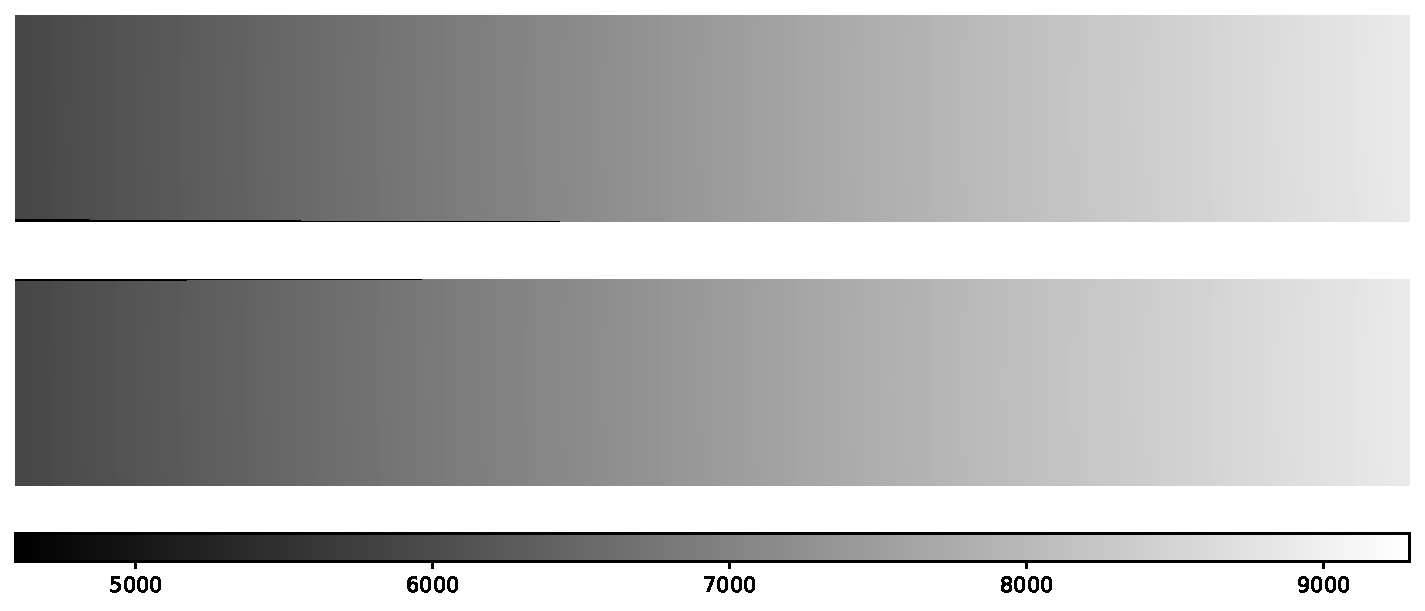
\includegraphics[width = 1.0\textwidth]{figures/3_pol_wav_ext.pdf}
    \caption{The wavelength extension of a \gls{FITS} file ready to be handed back to the \polsalt\ pipeline.}
    \label{fig:pol_wav_ext}
\end{figure}

% cosmic ray cleaning
\texttt{join} cleans the science extension of cosmic rays using the \texttt{lacosmic} python package which was specifically designed for this purpose and uses the L.A. Cosmic algorithm, based on Laplacian edge detection. The parameters used for cosmic ray cleaning were chosen based on the properties of the \gls{RSS}, specifically the read noise and gain, as well as a publication and \hyperlink{http://www.astro.yale.edu/dokkum/lacosmic/pars.html}{suggestions} by the algorithm's creator \citep{lacosmic}. The chosen parameters work well for all but the worst of cosmic rays, as can be seen when comparing Figures~\ref{fig:OE_split} and \ref{fig:polsalt_post_wav_cal}.
\prgph

% polsalt specific cropping (wav mask)
% mask wavelength using wollaston curve for polsalt `parsability'
% update BPM to reflect wavelength cropping
The wavelength extension is masked to remove any impossible wavelengths and also corrected for the skewing of the trace introduced by the wollaston element. The skewing must be added to the wavelength extension since \polsalt\ introduces a wollaston correction in the \texttt{spectra extraction} process. Finally, the \gls{BPM} extension is masked to reflect the valid wavelength calibrated regions for both spectropolarimetric beams and the files are saved with the \polsalt\ wavelength calibrated `wmxgbp' prefix.

\begin{figure}[t]
    \centering
    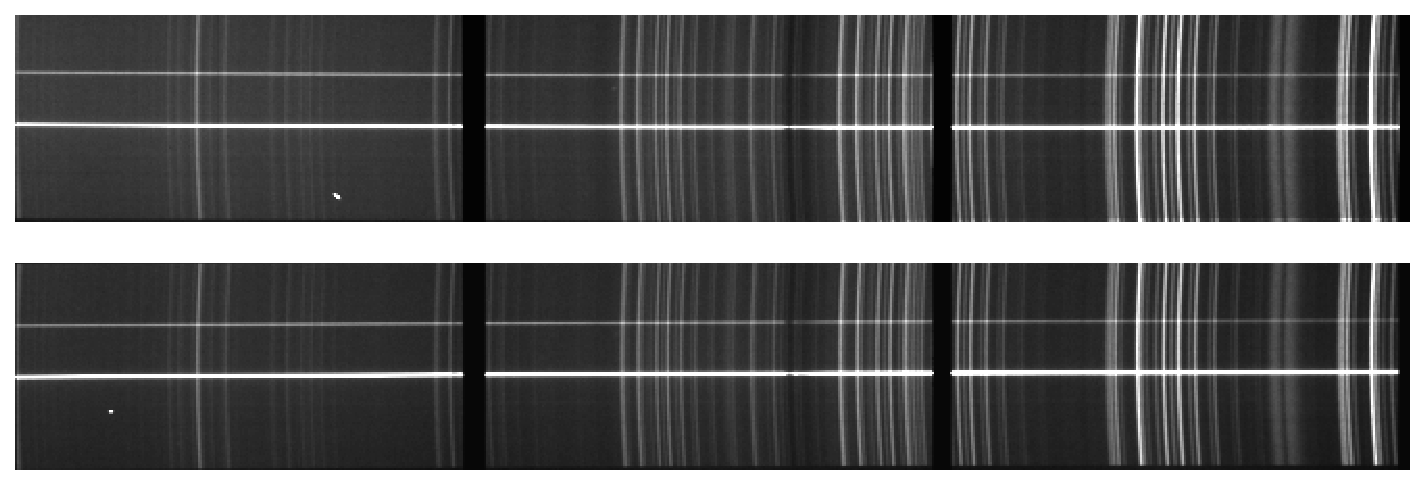
\includegraphics[width = 1.0\textwidth]{figures/3_post_wav_cal.pdf}
    \caption{The science extension of a \gls{FITS} file ready to be handed back to the \polsalt\ pipeline.}
    \label{fig:polsalt_post_wav_cal}
\end{figure}


\section{Additional Tools}\label{sec:add_tools}

Before creating the supplementary tool's \texttt{split} and \texttt{join} methods used to perform wavelength calibrations in \iraf, it was deemed necessary to create a tool to allow for the comparison of the wavelength solutions between the extracted spectra of the $O$ and $E$ polarization beams, referred to as \texttt{correlate}. The scope was later expanded to allow for the inspection of the cross-row and cross-column axes of the wavelength solutions as the \iraf\ wavelength calibration procedure provided much more flexibility.


\subsection{Sky line comparisons}\label{subsec:skyline_discuss}

Sky line comparisons serve two unique yet interconnected services. Firstly, they naively transform the wavelength calibrated frames, without conserving flux, allowing the user confirmation of the variation of sky lines across the columns of the frame, and secondly, they compare the wavelength position of the sky lines with the \gls{SALT} sky lines,\footnote{The first iteration of a sky line atlas is available at \url{https://astronomers.salt.ac.za/data/salt-longslit-line-atlas/}} allowing confirmation of the wavelength solution at positions across the rows of the frame. The file used for skyline comparisons may be the \iraf\ \texttt{transform} \gls{FITS} file, which allows for flux conservation through the `\texttt{flux}' parameter.
\prgph

The \texttt{skyline} method loads the wavelength calibrated files, transforms the frames (as described above) if the frame was not transformed by \iraf's \texttt{transform} method, divides out the continua, compares the cross-column sky lines to those of a single row, and compares the wavelength position of said sky lines to a list of sky lines known by \gls{SALT}.

Determining if there is an inaccuracy in the wavelength solution in the spatial ($y$, or vertical) axis is relatively straightforward as a perfect wavelength solution will remove any horizontal variation of the sky lines. Any horizontal deviation of the sky lines after transformation reflects a poor fit of the wavelength solution. Any vertical variation may be found through a quick visual inspection of a transformed frame, as mentioned previously, but may be inspected more thoroughly using the \texttt{skyline} method. As mentioned, the sky lines are averaged and compared to sky lines of a typical row. A wavelength solution exhibiting a poor fit across the spatial axis will display broader averaged sky lines than that of a relatively good fit.
\prgph

As no features, other than the trace of sources exposed across a frame, exist that uniformly cover the wavelength ($x$, horizontal) axis of a typical frame, determining if the horizontal fit of the wavelength solution is more challenging. Thankfully, \gls{SALT} has published a sky line atlas which we may make use of. By first considering the spatial fit of the wavelength solution, it is ensured that the wavelength positions of all sky lines are well-defined. Comparisons may now be made to the wavelength positions measured by \gls{SALT}. Minor variations in the comparison of the sky lines are expected, but any uniform trends indicate an underlying poor fit across the wavelength axis of the wavelength solution. A poor horizontal fit is difficult to spot without supplementary tools and may have drastic adverse effect on the final polarization results.


\subsection{Cross correlation}

The \texttt{skyline} method allows for confirmation of a single wavelength solution, but has no means for comparing how the wavelength solutions of two polarization beams differ from one another. The \texttt{correlate} method was created for this express purpose.
\prgph

Cross correlation of the two spectra allows for the comparison of the features within the spectra as a function of the wavelength displacement. This is useful when dealing with spectropolarimetric spectra as it allows a comparison of how well aligned the spectra are wavelength-wise. Using this, we can determine if any misidentifications had skewed the entire wavelength solution, as compared to the \texttt{skyline} method which allows identification of singular misidentifications within the wavelength solution.
\prgph



\todo{
    \begin{itemize}
        \item Why cross correlation
        \item discussion of script processes (how it works)
    \end{itemize}
}


\section{General Reduction Procedure}\label{sec:red_proc}

\begin{figure}[t]
    \centering
    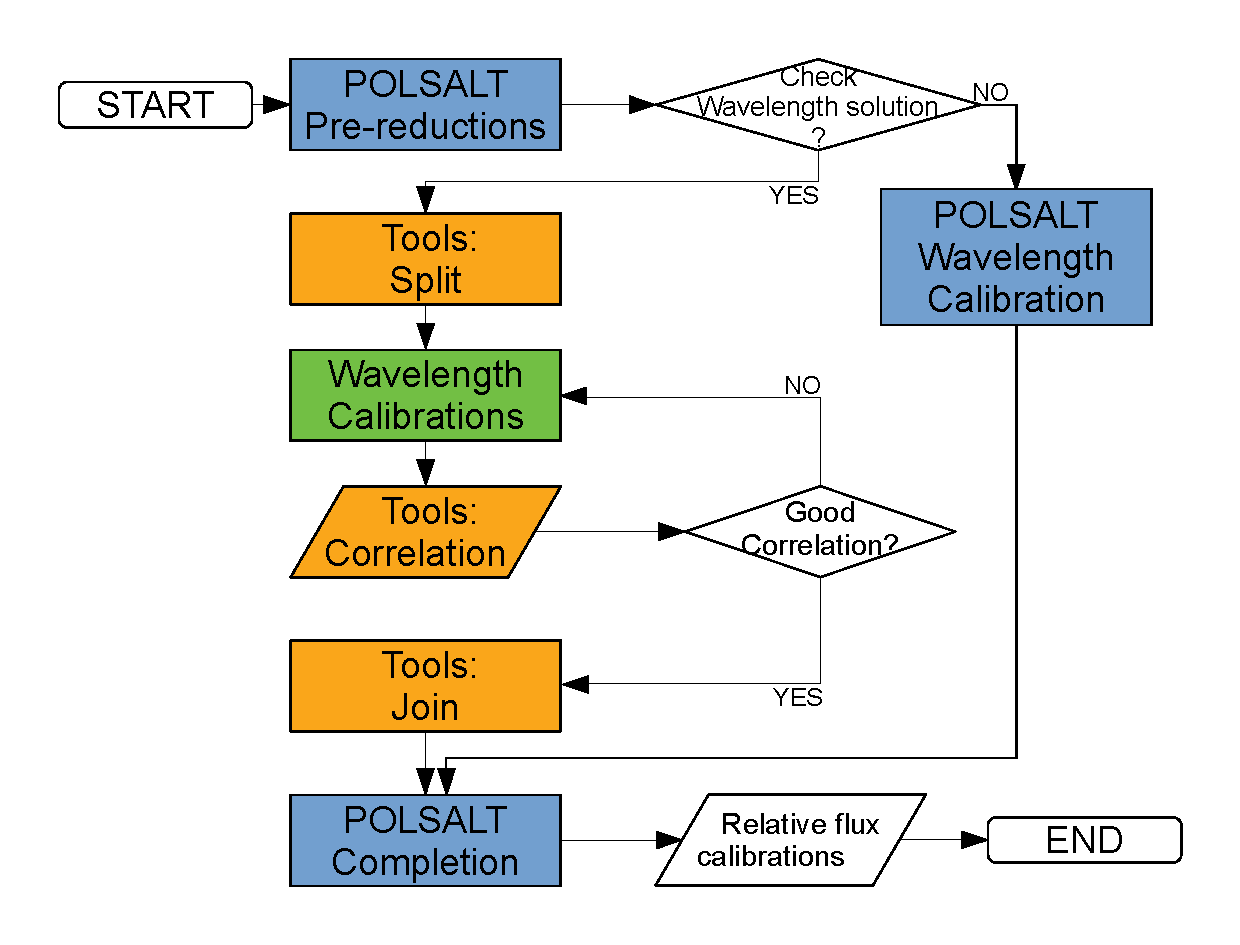
\includegraphics[width = 0.8\textwidth]{figures/3_new_workflow.pdf}
    \caption{A general workflow for data reductions using a combination of \polsalt, \iraf, and the developed supplementary tools.}
    \label{fig:new_workflow}
\end{figure}

This section aims to give an overview of the reduction procedure from start to finish and to cover all commands needed to achieve a finalized result. As users all employ a variety of operating systems, language environments, and software setups, not much emphasis will be placed on how to get the software running or the managing of files, only the commands necessary to complete each step of the reduction process, assuming that the software is running as intended.
\prgph

It is recommended that \polsalt\ is used through the \gls{GUI} as it provides a user-friendly environment while also sequentially listing each step of the reduction process in a dropdown menu. Reductions are possible, however, purely using a \gls{CLI} and the \polsalt\ scripts. It is assumed that usage of \polsalt\ through the \gls{GUI} or \gls{CLI} use the `beta' or `basic' versions, respectively, and that the beta version is launched from the \polsalt\ directory while the basic version is run by copying over the `scripts' folder to the working directory. The \iraf\ terminal, once launched, and the \gls{CLI} supplementary tools are also assumed to be run from the `working' directory. This ensures that commands containing \texttt{<.../>} notate the need for the inclusion of relative paths to the desired file or folder.
\prgph

Help documentation, primarily describing the possible arguments, is available in the \gls{CLI} for \polsalt\ and the supplementary tools using the \texttt{-h|--help} flag with their respective invocation, such as:

\begin{verbatim}> python <.../>Masters --help\end{verbatim}

\noindent and for \iraf\ through the \texttt{?|:.help} `cursor mode' options while running an interactive task.


\subsection{POLSALT Pre-reductions}\label{subsec:reduc_pre}

\polsalt\ requires a file structure such that the raw data received from \gls{SALT} is located in a folder labeled using the observing date as well as being in a sub-folder labeled raw, such as \texttt{YYYYMMDD/raw/}. This directory structure allows \polsalt\ to create a `working' directory named \texttt{YYYYMMDD/sci/} which contains all the files modified during the reduction process. This allows for separation of reductions of the same data by simply renaming the \texttt{sci/} directory.
\prgph

To launch the \gls{GUI}, navigate to the \polsalt\ directory within a \gls{CLI} and run:

\begin{verbatim}> python -W ignore reducepoldataGUI.py &\end{verbatim}

\noindent Once the window has launched, ensure that the first and second paths at the top of the window point to the \polsalt\ and data observation date directories, respectively. The `raw image reduction' may then be selected from the dropdown and run. The \polsalt\ \gls{CLI} command:

\begin{verbatim}> python scripts/reducepoldata.py <.../>YYYYMMDD\end{verbatim}

\noindent then runs the raw image reduction process. It should be noted that the \polsalt\ \gls{CLI} command will, by default, attempt to run the wavelength calibration process. This behavior may be stopped by using the \texttt{-w} flag when running the command.
\prgph

\todo{Include screenshot of GUI, reference in paragraph above}


\subsection{Wavelength Calibration} \label{subsec:reduc_wav}

The wavelength calibrations may now be completed in \iraf. This section concerns the procedure for parsing the \gls{FITS} files to be read by \iraf\ and \polsalt\ as well as the relevant task names and methods to be run to complete the calibrations. A base working case of each of the tasks and methods are presented below, but it should be noted that the art of wavelength calibration consists of modifying the parameters to achieve a good calibration function. This process depends heavily and varies greatly based on the user and as such not all use cases can be discussed herein.

\subsubsection{Preparing data for IRAF}

Splitting the data in the working \texttt{sci/} directory may then be done through a \gls{CLI} using:

\begin{verbatim}> python <.../>Masters split\end{verbatim}

The method takes multiple parameters, but default parameters are used where ever possible. The most notable parameters are the directory, which defaults to the current working directory of the \gls{CLI}, the split row, which defaults to \polsalt's default center row, and the save prefix, which defaults to `\texttt{obeam}' and `\texttt{ebeam}'. As an aside, the save prefix may be worth changing as, later in the reduction process, the \polsalt\ raw stokes reductions indiscriminately selects files named \texttt{YYYYMMDD/sci/e*.fits}.


\subsubsection{IRAF wavelength calibrations}

Moving on to \iraf, the wavelength calibrations are performed using the tasks described in \S~\ref{subsec:IRAF_wav_cal}, namely \texttt{identify}, \texttt{reidentify}, and \texttt{fitcoords}, and may be run directly in the \iraf\ terminal using:\footnote{Please see the \iraf\ help docs, available at \url{https://astro.uni-bonn.de/~sysstw/lfa_html/iraf/iraf.html}, on the relevant tasks for a comprehensive discussion of the parameters available.}

\begin{verbatim}
cl> identify images
cl> reidentify reference images
cl> fitcoords images fitname
\end{verbatim}

\noindent where `images' refer to a list or file containing the \gls{FITS} files relevant to the task, `reference' refers to the \gls{FITS} file previously identified, and `fitname' refers to the name to be used for the final two-dimensional wavelength solution. The interactive tasks take up the bulk of the reduction time as this is where the fine-tuning of the reduction is done, through the use of cursor commands (otherwise known as colon commands), which allow modification of the parameters mid-reduction. Task parameters may, however, be edited beforehand within the \iraf\ terminal using the \texttt{eparam} task, and optionally saved, and quit or run using a combination of \texttt{:w}, and \texttt{:q} or \texttt{:go} cursor commands, respectively.
\prgph

It is recommended to create an \iraf\ Command Language (cl) script for each task to keep track of which parameters were used and for simple recalibrations. The scripts are created using:

\begin{verbatim}cl> mkscript script_name.cl\end{verbatim}

\noindent which will interactively ask for the task and parameters to be used. Multiple tasks may be appended to an \iraf\ script, allowing for the parameters of both beams to be tracked. Running an \iraf\ script may be done by running:

\begin{verbatim}cl> cl < script_name.cl\end{verbatim}

\noindent but is not suggested for interactive scripts, which run best when simply copied from the \texttt{<.../>sci/script\_name.cl} file to the \iraf\ terminal.


\subsubsection{Preparing data for POLSALT}

The results of the wavelength calibrations may now be parsed back into the format expected by \polsalt. Joining the separate beams with their respective wavelength solutions is once again performed in the \gls{CLI} and is completed using:

\begin{verbatim}> python <.../>Masters join\end{verbatim}

Similar to the \texttt{split} procedure mentioned before, the \texttt{join} procedure has the same defaults defined and so it is up to a user to keep track of which defaults they decided to change and keep them consistent between the two tasks.


\subsubsection{Supplementary checks of the wavelength solution}

The supplementary tools and the optional \iraf\ \texttt{transform} task are used as methods for confirming the wavelength solutions across the frame, against reference wavelength positions, and across the polarization beams. They are all discussed here as this section pertains to the supplementary tools and \iraf\ procedures, but might only be used later on in the reduction process.
\prgph

The \iraf\ \texttt{transform} task may be run before closing the \iraf\ environment using:

\begin{verbatim}cl> transform images output fitnames\end{verbatim}

\noindent where `images' refers to the same pseudonym as used in the previous \iraf\ task usage examples, `output' refers to the new file name for the transformed input images, and `fitnames' refers to the two-dimensional wavelength function name created by the \texttt{fitcoords} task.
\prgph

The \texttt{skyline} method is run in the \gls{CLI} using:

\begin{verbatim}> python <.../>Masters skyline cal_images\end{verbatim}

\noindent where `cal\_images' refers to either the transformed images, prefixed `t', produced by the \iraf\ \texttt{transform} task or the raw wavelength calibrated frames. The difference in the flux conservation when \texttt{skyline} transforms the frames is discussed in \S~\ref{subsec:skyline_discuss}. Otherwise, as with all the other supplementary tools, default parameters also describe the overplotting of the $O$ and $E$ beams, the overplotting of the skylines provided by \gls{SALT}, and the cross row variation of a frame.
\prgph

The \texttt{correlate} method is run in the \gls{CLI} using:

\begin{verbatim}> python <.../>Masters correlate spec_images\end{verbatim}

\noindent where `spec\_images' refers to spectra extracted \gls{FITS} files. If the user wishes to compare the $O$ and $E$ beams of a single file then only that image name is to be provided, otherwise it is assumed that the user wishes to compare the same polarization beam across the files provided. It is worth pointing out here that as the input images are only created after performing the \polsalt\ \texttt{spectra extraction} and thus should only be completed thereafter.


\subsection{POLSALT Reduction Completion} \label{subsec:reduc_com}

Reductions may now be completed using \polsalt. The reduction process consists of correcting for the wollaston tilt, extracting the spectra, creating the stokes files, and displaying the results. As always, the reductions are handled slightly differently for the differing versions.

\subsubsection{POLSALT, the basic version}

Covering the basic version first, the wavelength solution needs to be applied to all the \gls{FITS} files and the tilt introduced by the wollaston prism must be corrected for. This is done through the command:

\begin{verbatim}> python scripts/correct_files.py w*fits\end{verbatim}

\noindent where the `w*.fits' is a wildcard expression that lists the \gls{FITS} files that have a wavelength extension and returns it to the \polsalt\ script.
\prgph

Next, the spectra in each \gls{FITS} file are extracted using the command:

\begin{verbatim}> python scripts/pol_extract.py c*.fits --yo A --ye B --dy C\end{verbatim}

\noindent where the center row of the $O$ and $E$ beam spectra, \texttt{A} and \texttt{B}, as well as the spectral width, \texttt{C}, are integer values and must be provided. These may be found through \gls{FITS} viewing software such as ds9\footnote{Available at \protect\url{https://sites.google.com/cfa.harvard.edu/saoimageds9}} or more manually through python.
\prgph

The Stokes files may then be calculated and created using the command:

\begin{verbatim}> python scripts/pol_stokes.py\end{verbatim}

\noindent which automatically detects the \gls{FITS} files using the wildcards `e*fits' for raw stokes and `*\_h*.fits' for the final stokes calculations. The deletion of the \gls{FITS} files created in the supplementary \texttt{split} method may be deleted in the \texttt{join} method specifically to avoid this naming convention clash, but may also be avoided by providing an alternate default subscript to the supplementary methods.
\prgph

Finally, the results of the stokes calculations may be viewed using the command:

\begin{verbatim}> python polsalt/specpolview.py *_stokes.fits\end{verbatim}

\noindent where a file name, which may also use a wildcard, is provided as well as optional para\-meters to define the binning (\texttt{bin=[int]A} where [int] refers to an actual integer value), error bars (\texttt{errors=True|False}), choice of plot (\texttt{type=Ipt|Iqu} for unbinned intensity and either polarization percentage and polarization angle, or $Q$ and $U$ stokes parameters), save options (\texttt{save=[text][plot] where either or both `text' and `plot' may be provided}), and a debug mode (\texttt{debug=False|True}).


\subsubsection{POLSALT, the beta version}

The \polsalt\ beta version has access to a \gls{GUI} but may also be run as a script. The script will be discussed before the \gls{GUI} as it is straightforward to run and modify.
\prgph

Firstly, to run the \polsalt\ beta script, it is suggested to copy over the \texttt{reducepol\-data\_sc.py} to the working directory. In general, running the script as:

\begin{verbatim}> python reducepoldata_sc.py YYYYMMDD\end{verbatim}

\noindent will run the entire reduction process interactively without the need to select which process to run next. For the purposes of using the script alongside \iraf\ wavelength calibrations, a few changes must be made. The script may either be run with a break inserted before the call to the wavelength calibration, \texttt{specpolwavmap}, and later rerun with all processes before spectral extraction, \texttt{specpolextract\_sc}, commented out, or may be split into two seperate files which cover the pre- and post- wavelength calibration steps and run when appropriate.
\prgph

The \polsalt\ beta \texttt{reducepoldata\_sc.py} copies a \texttt{script.py} file into the science working directory, `YYYYMMDD/sci/', which provides analysis scripts for analysis and modification of the \polsalt\ beta results. These tools consist of data culling for the final stokes calculations, text and plot output (the same as the basic version of \polsalt's \texttt{specpolview.py}), relative flux calibration corrections, and synthetic filtering of polarization results. The \polsalt\ analysis scripts may be run using:

\begin{verbatim}> python script.py\end{verbatim}

\noindent followed by \texttt{specpolfinalstokes.py}, \texttt{specpolview.py}, \texttt{specpolflux.py}, or \texttt{specpol\-filter.py}, respectively, for the analysis modes mentioned previously. Each mode has its own usage parameters, and it is suggested that a user look up the documentation before attempting to use any of them.\footnote{A description of the use of each analysis script is available from \url{https://github.com/saltastro/polsalt/wiki/Linear-Polarization-Reduction.--Beta-version} and is exhaustive enough for general use, but the source code is also made available and should be consulted before usage.}
\prgph

Finally, the reduction process using the \polsalt\ \gls{GUI} is completed by selecting and, when applicable, interactively modifying the reduction step through the interactive windows, one-by-one, from the \glspl{GUI} dropdown menu.
\prgph

\todo{
    \begin{itemize}
        \item Deletion of o and e beam fits (due to POLSALT naming conventions and to save memory)
        \item finish GUI write-up
    \end{itemize}
}